\section{Auswertung}
\label{sec:Auswertung}

\begin{figure}
  \centering
  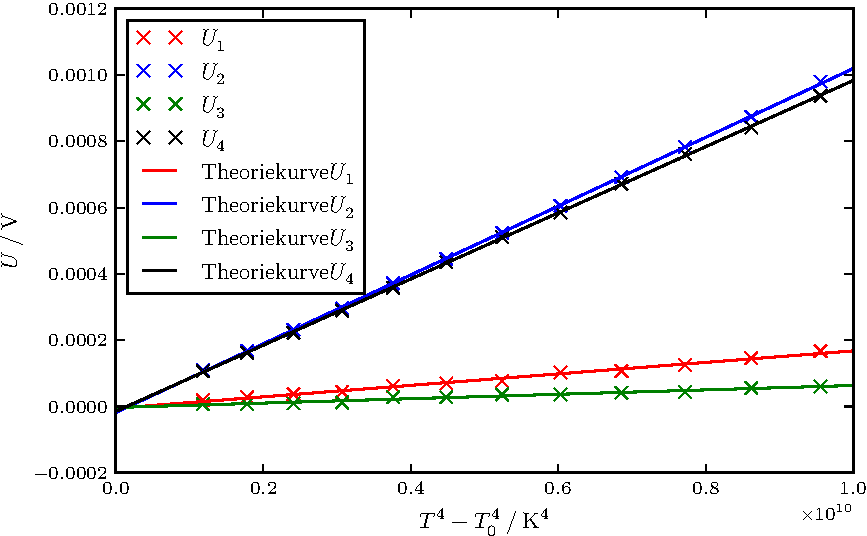
\includegraphics{plot.pdf}
  \caption{Plot.}
  \label{fig:plot}
\end{figure}
Die gemessenen Daten für die Tempeatur $T_1$ des wärmeren sowie die Temperatur
$T_2$ des kälteren Reservoirs wurden gegen die Zeit $t$ in Minuten abgetragen.
Mithilfe von SciPy wurde jeweils eine Ausgleichsgerade für die folgende Funktion
berechnet:
\begin{equation}
  T(t)=A \cdot t^2 + B \cdot t + C
\end{equation}
Die Parameter $A$, $B$ und $C$ wurden bestimmt zu
\begin{align}
  A_{T_1} &= -0.01395 & B_{T_1} &= 1.40708 & C_{T_1} &= 293.592 \\
  A_{T_2} &= 0.01566  & B_{T_2} &= -1.08915 & C_{T_2} &= 294.936
\end{align}
